\documentclass[]{article}

% Imported Packages
%------------------------------------------------------------------------------
\usepackage{amssymb}
\usepackage{amstext}
\usepackage{amsthm}
\usepackage{amsmath}
\usepackage{enumerate}
\usepackage{fancyhdr}
\usepackage[margin=1in]{geometry}
\usepackage{graphicx}
\usepackage{extarrows}
\usepackage{setspace}
\usepackage{graphicx}
\graphicspath{ {./asset/} }
%------------------------------------------------------------------------------

% Header and Footer
%------------------------------------------------------------------------------
\pagestyle{plain}  
\renewcommand\headrulewidth{0.4pt}                                      
\renewcommand\footrulewidth{0.4pt}                                    
%------------------------------------------------------------------------------

% Title Details
%------------------------------------------------------------------------------
\title{Deliverable \#1 Template}
\author{SE 3A04: Software Design II -- Large System Design}
\date{}                               
%------------------------------------------------------------------------------

% Document
%------------------------------------------------------------------------------
\begin{document}

\maketitle	

\section{Introduction}
\label{sec:introduction}
% Begin Section

This section of the SRS should provide an overview of the entire SRS.

\subsection{Purpose}
\label{sub:purpose}
% Begin SubSection
\begin{enumerate}[a)]
	\item Delineate the purpose of the SRS
	\item Specify the intended audience for the SRS
\end{enumerate}
% End SubSection

\subsection{Scope}
\label{sub:scope}
% Begin SubSection
\begin{enumerate}[a)]
	\item Identify the software product(s) to be produced by name (e.g., Host DBMS, Report Generator, etc.)
	\item Explain what the software product(s) will, and, if necessary, will not do
	\item Describe the application of the software being specified, including relevant benefits, objectives, and goals
	\item Be consistent with similar statements in higher-level specifications (e.g., the system requirements specification), if they exist
\end{enumerate}
% End SubSection

\subsection{Definitions, Acronyms, and Abbreviations}
\label{sub:definitions_acronyms_and_abbreviations}
% Begin SubSection
\begin{enumerate}[a)]
	\item Provide the definitions of all terms, acronyms, and abbreviations required to properly interpret the SRS
\end{enumerate}
% End SubSection

\subsection{References}
\label{sub:references}
% Begin SubSection
\begin{enumerate}[a)]
	\item Provide a complete list of all documents referenced elsewhere in the SRS
	\item Identify each document by title, report number (if applicable), date, and publishing organization
	\item Specify the sources from which the references can be obtained
\end{enumerate}
% End SubSection

\subsection{Overview}
\label{sub:overview}
% Begin SubSection
\begin{enumerate}[a)]
	\item Describe what the rest of the SRS contains
	\item Explain how the SRS is organized
\end{enumerate}
% End SubSection

% End Section

\section{Overall Description}
\label{sec:overall_description}
% Begin Section

This section of the SRS should describe the general factors that affect the product and its requirements. It does not state specific requirements; it provides a background for those requirements and makes them easier to understand.

\subsection{Product Perspective}
\label{sub:product_perspective}
% Begin SubSection
\begin{enumerate}[a)]
	\item The product being developed is an Android application which empowers the ability to book carpool via a user-friendly interface using a taxi company. The application will securely store customer personal information such as carpool request histories, and personal data inputted by the user. The product is not self-contained since its functionality depends heavily on the taxi service provider. There are several out-of-scope concerns such as: driver\textquotesingle s information input (profile, shift, locations, etc.) and payment processing.
	\item The general interaction can be visualized as follows: 
	\begin{center}
		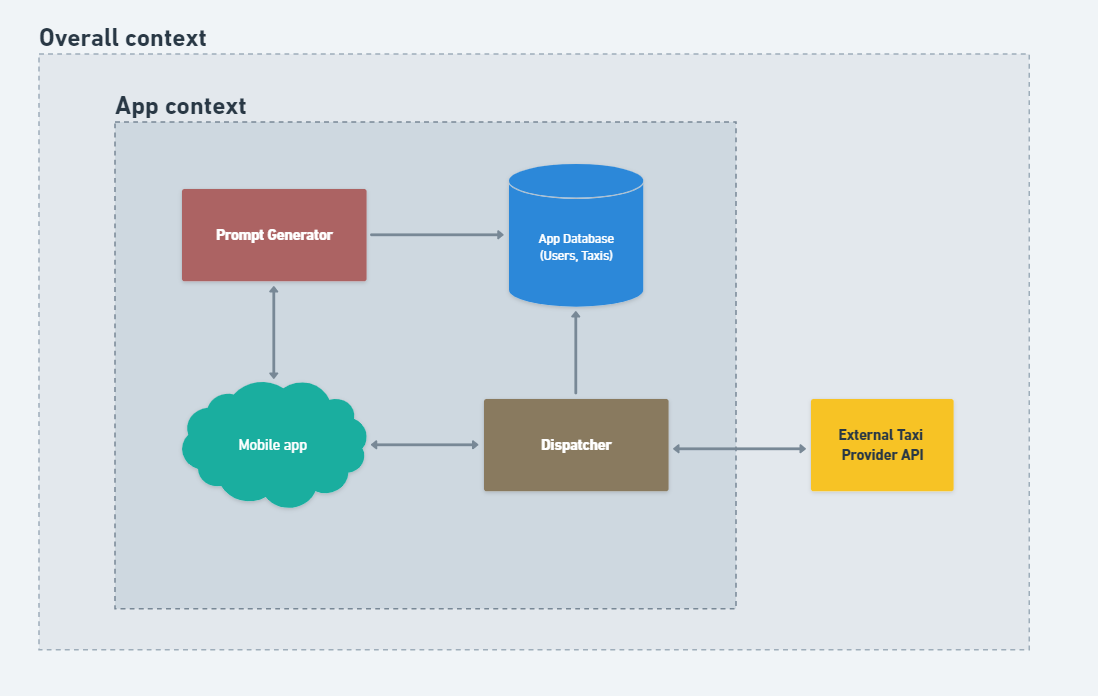
\includegraphics[scale=0.5]{app-context.png}
	\end{center}
\end{enumerate}
% End SubSection

\subsection{Product Functions}
\label{sub:product_functions}
% Begin SubSection
	\begin{center}
		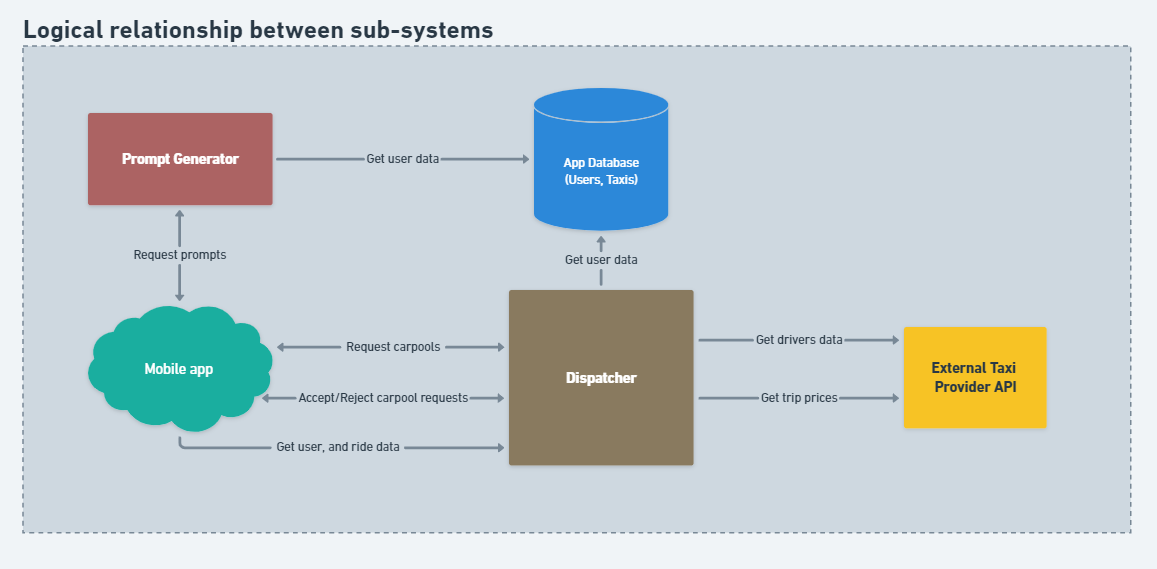
\includegraphics[scale=0.5]{subsys-relationship.png}
	\end{center}

\begin{enumerate}[a)]
	\item The app will be able to book taxi.
	\begin{itemize}
		\item Able to communicate with taxi\textquotesingle s service API.
		\item Able to handle and display taxi data correctly.	
	\end{itemize}
	\item The app be able to handle carpool scheduling and coordination.
	\begin{itemize}
		\item Able to plan the most optimal route and let the driver follow the calculated route.
	\end{itemize}
	\item The app be able to display the estimate time-of-arrival (ETA) of taxis.
	\begin{itemize}
		\item Able to calculate ETA in real-time
	\end{itemize}
	\item The app be able to input the taxi\textquotesingle s unique identifier via the mobile app.
\end{enumerate}
% End SubSection

\subsection{User Characteristics}
\label{sub:user_characteristics}
% Begin SubSection
\begin{enumerate}[a)]
	\item Riders
	\begin{itemize}
		\item Riders are users who use the app to request car pool.
		\item Riders can be anyone from any background of tech-expertise
		\item Riders are expected to:
		\begin{itemize}
			\item Input personal information only a few times.
			\item Have stable and highly available mobile internet connection.
		\end{itemize}
		
		\item Riders might be interested one or more following characteristics of the app:
		\begin{itemize}
			\item User interface and experience of navigating the mobile app.
			\item Realtime taxi information display (ETA, location, route, …)
			\item Ease of taxi booking, and check-in.  
		\end{itemize}
	\end{itemize}
	
	\item Taxi Drivers
	\begin{itemize}
		\item Drivers are users who drive and operate taxis, fulfill carpool requests, and ensure the safety of the riders.
		\item Drivers must be registered with the taxi service and from any background of tech-expertise.  
		\item Drivers are expected to have stable and highly available mobile internet connection.
		\item Drivers might be interested one or more following characteristics of the app:
		\begin{itemize}
			\item Accuracy display of real-time pick-up and drop-off information.
			\item Accuracy of aggregating and storing of rides information (since it ties directly to their performance).
			\item Accuracy display of user\textquotesingle s profile summarization.
			\item User interface and experience of navigating the mobile app.
			\item Ease of accepting/ rejecting rides.
		\end{itemize}

	\end{itemize}

\end{enumerate}
% End SubSection

\subsection{Constraints}
\label{sub:constraints}
% Begin SubSection
\begin{enumerate}[a)]
	\item \textbf{Geographical}: The app can only operate on the land which the taxi service operate.
	\item \textbf{Technological}: App must be integrated with softwares that the taxi service provider uses.
	\item \textbf{Fare Determination}: Since the app does\textquotesingle t support payment processing directly, the fare has to be determined and processed through the taxi service provider.
	\item \textbf{Data Privacy Regulation}: Data which transmits and stored within the app needs to be processed in a way which complies with the data protection act.

\end{enumerate}
% End SubSection

\subsection{Assumptions and Dependencies}
\label{sub:assumptions_and_dependencies}
% Begin SubSection
\begin{enumerate}[a)]
	\item Assumptions
	\begin{itemize}
		\item Drivers information are provided by the taxi provider (driver profile and shift).
		\item The taxi provider has dedicated API which provide real-time data on driver\textquotesingle s availability.
		\item The taxi provider determines trip prices.
		\item Payment processing is external and not under the scope of the application.

	\end{itemize}

	\item Many problems may occur when the following assumptions failed to hold:
	\begin{itemize}
		\item If trip prices are not determined by the taxi service provider, additional calculations must be performed to find fare fees after each trip.
		\item If drivers data are stored and handled within the context of the app, additional mechanism must be provided for drivers to update their information. In addition, driver\textquotesingle s data storage must comply with the Canadian Data Protection Act. 


	\end{itemize}
\end{enumerate}
% End SubSection

\subsection{Apportioning of Requirements}
\label{sub:apportioning_of_requirements}
% Begin SubSection
\begin{enumerate}[a)]
	\item \textbf{Technological}: Some specific technilogical requirements (Database type, Integration with taxi provider, etc...) have to be delayed untill the implementation phase.
	\item Non-function Requiremens such as UI,UX, or performance can be finetuned when the app is being implemented or after release.
\end{enumerate}
% End SubSection

% End Section

\section{Use Case Diagram}
\label{sec:use_case_diagram}
% Begin Section
This section should provide a use case diagram for your application. 
\begin{enumerate}[a)]
	\item Each use case appearing in the diagram should be accompanied by a text description. 
\end{enumerate}
% End Section

\section{Functional Requirements}
\label{sec:functional_requirements}
% Begin Section
This section of the SRS should contain all of the software requirements to a level of detail sufficient to enable designers to design a system to satisfy those requirements, and testers to test that the system satisfies those requirements. Throughout this section, every stated requirement should be externally perceivable by users, operators, or other external systems. These requirements should include at a minimum a description of every input (stimulus) into the system, every output (response) from the system, and all functions performed by the system in response to an input or in support of an output.

You normally have two options for organizing your functional requirements:
\begin{enumerate}
	\item Organize first by \emph{business events}, then by \emph{viewpoints}
	\item Organize first by \emph{viewpoints}, then by \emph{business events}
\end{enumerate}
Choose the one which makes the most sense.

For example, if you wish to organization by business events:
\begin{enumerate}[{BE}1.]
	\item Business Event
	\begin{enumerate}[{VP1}.1]
		\item Viewpoint
			\begin{enumerate}
				\item Requirement
				\item Requirement
				\item \dots
			\end{enumerate}
		\item Viewpoint
			\begin{enumerate}
				\item Requirement
				\item Requirement
				\item \dots
			\end{enumerate}
		\item \dots
	\end{enumerate}
	\item Business Event
	\begin{enumerate}[{VP2}.1]
		\item Viewpoint
			\begin{enumerate}
				\item Requirement
				\item Requirement
				\item \dots
			\end{enumerate}
		\item Viewpoint
			\begin{enumerate}
				\item Requirement
				\item Requirement
				\item \dots
			\end{enumerate}
		\item \dots
	\end{enumerate}
\end{enumerate}

\underline{OR}, if you wish to organization by viewpoints:
\begin{enumerate}[{VP}1.]
	\item Viewpoint 
	\begin{enumerate}[{BE1}.1]
		\item Business Event
		\begin{enumerate}
			\item Requirement
			\item Requirement
			\item \dots
		\end{enumerate}
		\item Business Event
		\begin{enumerate}
			\item Requirement
			\item Requirement
			\item \dots
		\end{enumerate}
		\item \dots
	\end{enumerate}
	\item Viewpoint
	\begin{enumerate}[{BE2}.1]
		\item Business Event
		\begin{enumerate}
			\item Requirement
			\item Requirement
			\item \dots
		\end{enumerate}
		\item Business Event
		\begin{enumerate}
			\item Requirement
			\item Requirement
			\item \dots
		\end{enumerate}
		\item \dots
	\end{enumerate}
\end{enumerate}

% End Section

\section{Non-Functional Requirements}
\label{sec:non-functional_requirements}
% Begin Section
\subsection{Look and Feel Requirements}
\label{sub:look_and_feel_requirements}
% Begin SubSection

\subsubsection{Appearance Requirements}
\label{ssub:appearance_requirements}
% Begin SubSubSection
\begin{enumerate}[{LF}1. ]
	\item 
\end{enumerate}
% End SubSubSection

\subsubsection{Style Requirements}
\label{ssub:style_requirements}
% Begin SubSubSection
\begin{enumerate}[{LF}1. ]
	\item 
\end{enumerate}
% End SubSubSection

% End SubSection

\subsection{Usability and Humanity Requirements}
\label{sub:usability_and_humanity_requirements}
% Begin SubSection

\subsubsection{Ease of Use Requirements}
\label{ssub:ease_of_use_requirements}
% Begin SubSubSection
\begin{enumerate}[{UH}1. ]
	\item 
\end{enumerate}
% End SubSubSection

\subsubsection{Personalization and Internationalization Requirements}
\label{ssub:personalization_and_internationalization_requirements}
% Begin SubSubSection
\begin{enumerate}[{UH}1. ]
	\item 
\end{enumerate}
% End SubSubSection

\subsubsection{Learning Requirements}
\label{ssub:learning_requirements}
% Begin SubSubSection
\begin{enumerate}[{UH}1. ]
	\item 
\end{enumerate}
% End SubSubSection

\subsubsection{Understandability and Politeness Requirements}
\label{ssub:understandability_and_politeness_requirements}
% Begin SubSubSection
\begin{enumerate}[{UH}1. ]
	\item 
\end{enumerate}
% End SubSubSection

\subsubsection{Accessibility Requirements}
\label{ssub:accessibility_requirements}
% Begin SubSubSection
\begin{enumerate}[{UH}1. ]
	\item 
\end{enumerate}
% End SubSubSection

% End SubSection

\subsection{Performance Requirements}
\label{sub:performance_requirements}
% Begin SubSection

\subsubsection{Speed and Latency Requirements}
\label{ssub:speed_and_latency_requirements}
% Begin SubSubSection
\begin{enumerate}[{PR}1. ]
	\item 
\end{enumerate}
% End SubSubSection

\subsubsection{Safety-Critical Requirements}
\label{ssub:safety_critical_requirements}
% Begin SubSubSection
\begin{enumerate}[{PR}1. ]
	\item 
\end{enumerate}
% End SubSubSection

\subsubsection{Precision or Accuracy Requirements}
\label{ssub:precision_or_accuracy_requirements}
% Begin SubSubSection
\begin{enumerate}[{PR}1. ]
	\item 
\end{enumerate}
% End SubSubSection

\subsubsection{Reliability and Availability Requirements}
\label{ssub:reliability_and_availability_requirements}
% Begin SubSubSection
\begin{enumerate}[{PR}1. ]
	\item 
\end{enumerate}
% End SubSubSection

\subsubsection{Robustness or Fault-Tolerance Requirements}
\label{ssub:robustness_or_fault_tolerance_requirements}
% Begin SubSubSection
\begin{enumerate}[{PR}1. ]
	\item 
\end{enumerate}
% End SubSubSection

\subsubsection{Capacity Requirements}
\label{ssub:capacity_requirements}
% Begin SubSubSection
\begin{enumerate}[{PR}1. ]
	\item 
\end{enumerate}
% End SubSubSection

\subsubsection{Scalability or Extensibility Requirements}
\label{ssub:scalability_or_extensibility_requirements}
% Begin SubSubSection
\begin{enumerate}[{PR}1. ]
	\item 
\end{enumerate}
% End SubSubSection

\subsubsection{Longevity Requirements}
\label{ssub:longevity_requirements}
% Begin SubSubSection
\begin{enumerate}[{PR}1. ]
	\item 
\end{enumerate}
% End SubSubSection

% End SubSection

\subsection{Operational and Environmental Requirements}
\label{sub:operational_and_environmental_requirements}
% Begin SubSection

\subsubsection{Expected Physical Environment}
\label{ssub:expected_physical_environment}
% Begin SubSubSection
\begin{enumerate}[{OE}1. ]
	\item 
\end{enumerate}
% End SubSubSection

\subsubsection{Requirements for Interfacing with Adjacent Systems}
\label{ssub:requirements_for_interfacing_with_adjacent_systems}
% Begin SubSubSection
\begin{enumerate}[{OE}1. ]
	\item 
\end{enumerate}
% End SubSubSection

\subsubsection{Productization Requirements}
\label{ssub:productization_requirements}
% Begin SubSubSection
\begin{enumerate}[{OE}1. ]
	\item 
\end{enumerate}
% End SubSubSection

\subsubsection{Release Requirements}
\label{ssub:release_requirements}
% Begin SubSubSection
\begin{enumerate}[{OE}1. ]
	\item 
\end{enumerate}
% End SubSubSection

% End SubSection

\subsection{Maintainability and Support Requirements}
\label{sub:maintainability_and_support_requirements}
% Begin SubSection

\subsubsection{Maintenance Requirements}
\label{ssub:maintenance_requirements}
% Begin SubSubSection
\begin{enumerate}[{MS}1. ]
	\item 
\end{enumerate}
% End SubSubSection

\subsubsection{Supportability Requirements}
\label{ssub:supportability_requirements}
% Begin SubSubSection
\begin{enumerate}[{MS}1. ]
	\item 
\end{enumerate}
% End SubSubSection

\subsubsection{Adaptability Requirements}
\label{ssub:adaptability_requirements}
% Begin SubSubSection
\begin{enumerate}[{MS}1. ]
	\item 
\end{enumerate}
% End SubSubSection

% End SubSection

\subsection{Security Requirements}
\label{sub:security_requirements}
% Begin SubSection

\subsubsection{Access Requirements}
\label{ssub:access_requirements}
% Begin SubSubSection
\begin{enumerate}[{SR}1. ]
	\item 
\end{enumerate}
% End SubSubSection

\subsubsection{Integrity Requirements}
\label{ssub:integrity_requirements}
% Begin SubSubSection
\begin{enumerate}[{SR}1. ]
	\item 
\end{enumerate}
% End SubSubSection

\subsubsection{Privacy Requirements}
\label{ssub:privacy_requirements}
% Begin SubSubSection
\begin{enumerate}[{SR}1. ]
	\item 
\end{enumerate}
% End SubSubSection

\subsubsection{Audit Requirements}
\label{ssub:audit_requirements}
% Begin SubSubSection
\begin{enumerate}[{SR}1. ]
	\item 
\end{enumerate}
% End SubSubSection

\subsubsection{Immunity Requirements}
\label{ssub:immunity_requirements}
% Begin SubSubSection
\begin{enumerate}[{SR}1. ]
	\item 
\end{enumerate}
% End SubSubSection

% End SubSection

\subsection{Cultural and Political Requirements}
\label{sub:cultural_and_political_requirements}
% Begin SubSection

\subsubsection{Cultural Requirements}
\label{ssub:cultural_requirements}
% Begin SubSubSection
\begin{enumerate}[{CP}1. ]
	\item 
\end{enumerate}
% End SubSubSection

\subsubsection{Political Requirements}
\label{ssub:political_requirements}
% Begin SubSubSection
\begin{enumerate}[{CP}1. ]
	\item 
\end{enumerate}
% End SubSubSection

% End SubSection

\subsection{Legal Requirements}
\label{sub:legal_requirements}
% Begin SubSection

\subsubsection{Compliance Requirements}
\label{ssub:compliance_requirements}
% Begin SubSubSection
\begin{enumerate}[{LR}1. ]
	\item 
\end{enumerate}
% End SubSubSection

\subsubsection{Standards Requirements}
\label{ssub:standards_requirements}
% Begin SubSubSection
\begin{enumerate}[{LR}1. ]
	\item 
\end{enumerate}
% End SubSubSection

% End SubSection

% End Section

\appendix
\section{Division of Labour}
\label{sec:division_of_labour}
% Begin Section
Include a Division of Labour sheet which indicates the contributions of each team member. This sheet must be signed by all team members.
% End Section

\newpage
\section*{IMPORTANT NOTES}
\begin{itemize}
	\item Be sure to include all sections of the template in your document regardless whether you have something to write for each or not
	\begin{itemize}
		\item If you do not have anything to write in a section, indicate this by the \emph{N/A}, \emph{void}, \emph{none}, etc.
	\end{itemize}
	\item Uniquely number each of your requirements for easy identification and cross-referencing
	\item Highlight terms that are defined in Section~1.3 (\textbf{Definitions, Acronyms, and Abbreviations}) with \textbf{bold}, \emph{italic} or \underline{underline}
	\item For Deliverable 1, please highlight, in some fashion, all (you may have more than one) creative and innovative features. Your creative and innovative features will generally be described in Section~2.2 (\textbf{Product Functions}), but it will depend on the type of creative or innovative features you are including.
\end{itemize}


\end{document}
%------------------------------------------------------------------------------